
% Due Date: 6/15/14

\chapter{The Legion Runtime Architecture}
\label{chapter:arch}
Having completed our discussion of the Legion
programming model in Chapter~\ref{chapter:model},
we begin in earnest describing our implementation 
of Legion. Legion is currently implemented entirely 
as a runtime system. We decided on a runtime implementation 
for two reasons. First, a runtime system is fully dynamic 
and requires no static analysis of programs, thereby allowing 
it to react to the dynamic nature of both modern 
supercomputing applications and hardware. Second, 
implementing Legion as a runtime system in an existing 
language (in this case C++) makes it easier for application 
developers and DSL compiler writers to port their code as 
they are  already familiar with the target language and simply 
need to adapt to the new programming model.

Before delving into the details of our implementation
we begin with a brief overview of the various
components of the current Legion ecosystem in
Section~\ref{sec:components}.  We then introduce
a useful analogy in Section~\ref{sec:framework}
for describing how the Legion runtime system operates
that will be carried through many of the following
chapters.

\section{Runtime Organization}
\label{sec:components}
Due to the complex nature of both applications and
the underlying hardware, the Legion runtime is composed
of several different components at different levels of
abstraction. Figure~\ref{fig:softwarestack} illustrates
the different levels of the Legion software stack, 
including several levels (such as the Legion language
and compiler) that are still under development. 
The many different layers are designed to encapsulate
the complexity associated with the various aspects of 
our Legion implementation. We now discuss each of the 
different levels of the software stack in further detail.

\begin{figure}[ht]
\begin{center}
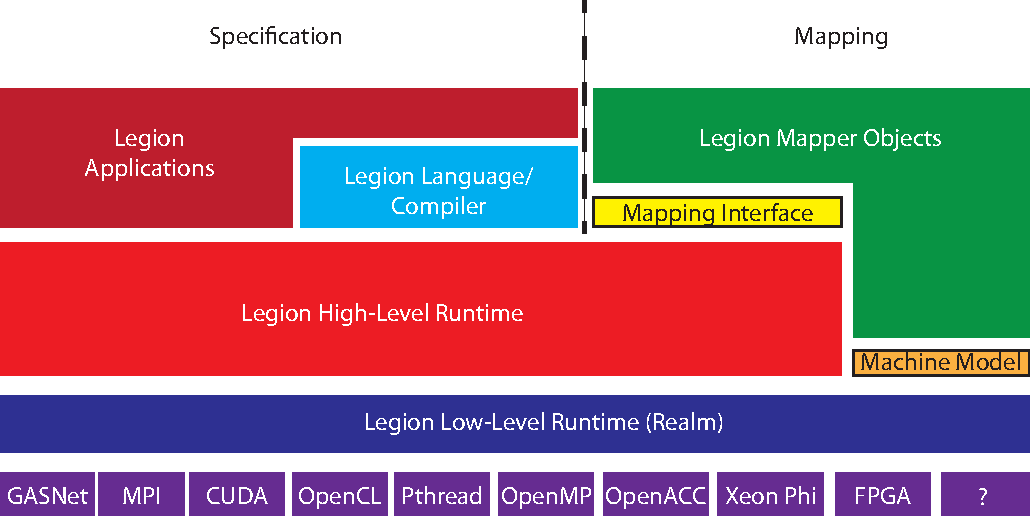
\includegraphics[scale=0.6]{figs/LegionSoftwareStack.pdf}
\end{center}
\caption{Legion Software Stack\label{fig:softwarestack}}
\end{figure}

\subsection{Legion Applications}
\label{subsec:legionapps}
At the top of Figure~\ref{fig:softwarestack} are Legion
applications. Legion applications can be either applications
directly written using Legion or Domain Specific Languages
and Libraries (DSLs) that use Legion to provide additional
portability and performance. Legion applications can be
targeted either at the Legion runtime API or at the 
higher-level Legion language developed in \cite{LegionTypes13}.
The design and implementation of the Legion language,
type system, and compiler are beyond the scope of this
thesis and are not discussed further.  From this point
forward we will assume all Legion applications make 
use of the Legion runtime API.

Included in Figure~\ref{fig:softwarestack} is a dividing
line that delineates which components of the Legion software 
stack apply to writing machine-independent specifications
and which apply to determining the best ways of
mapping applications onto a target architecture.
The features discussed in Chapter~\ref{chapter:model}
are used entirely for writing machine independent specifications
of applications. Alternatively, the features of the 
Legion mapping interface, that are covered in detail in
Chapter~\ref{chapter:mapping}, are entirely contained 
on the right side of this divide. The line dividing the
machine independent specification of an application from
its mapping does not extend beyond the application/mapper
level because it is the responsibility of the Legion
runtime to mediate the interaction between
machine-independent application specifications and
the mapping decisions made by mapper objects.

\subsection{High-Level Runtime}
\label{subsec:highlevel}
The Legion high-level runtime is an implementation
of the Legion programming model described in 
Chapter~\ref{chapter:model}. Our current implementation
of Legion supports a C++ interface for writing Legion
programs. While applications are written in C++, they
are required to abide by the Legion programming model.
Therefore, tasks are permitted to only access data
in regions that they request, all sub-tasks must be
launched through the runtime interface, and global
variables along with dynamic memory allocation are 
not permitted (logical regions are used instead).

It is the responsibility of the Legion high-level 
runtime to take applications written in the Legion 
programming model and convert them into the primitive
operations supplied by the low-level runtime interface
discussed in Section~\ref{subsec:lowlevel}. The 
mechanisms by which the high-level runtime performs this
transformation are the primary technical contributions
of this work. We begin our technical description of the
high-level runtime in Section~\ref{sec:framework}.

The other responsibility of the high-level runtime is
to mediate calls to mapper objects through the mapper
interface. As an application is executing, many decisions
need to be made regarding where tasks should be assigned
and where physical instances of logical regions should be 
placed. The high-level runtime directs these queries to the 
appropriate mapper object through the Legion mapper
interface\footnote{In this way the mapper interface is actually 
a call-back interface where methods of the mapper objects 
are invoked by the runtime.}.  Using the results of the 
mapping calls, the high-level runtime then carries out 
the specified mapping of an application onto the 
target architecture.

\subsection{Low-Level Runtime}
\label{subsec:lowlevel}
The design and implementation of the Legion low-level
runtime is covered in detail in \cite{Realm14} and is
mostly beyond the scope of this thesis.  However, we
briefly cover the important details of the low-level
runtime interface necessary for understanding the
interaction with the high-level runtime. 

The low-level runtime interface provides a useful set
of primitives for orchestrating computation, data
movement, and synchronization in a distributed memory
system. Specifically, it provides the following 
primitive operations:

\begin{itemize}
\item Tasks - launch tasks on specific processors either
              on local or remote nodes
\item Instances - allocate and free physical instances
                  in memories 
\item Copies - issue copies or reductions between physical instances
\item Synchronization - provide {\em reservations} as an 
                        atomicity primitive
\end{itemize}

The most important aspect of the low-level runtime is
that all of these primitives are non-blocking.
All operations are asynchronous and return
immediately with an {\em event} that names a time in the
future when the operation will be complete.  Furthermore
all operations in the low-level runtime can take
events as preconditions that are required to trigger before 
an operation can be executed. By using events to compose
these primitives, the high-level runtime can construct
large directed acyclic graphs (DAGs) of operations.

\begin{figure}[ht!]
\centering
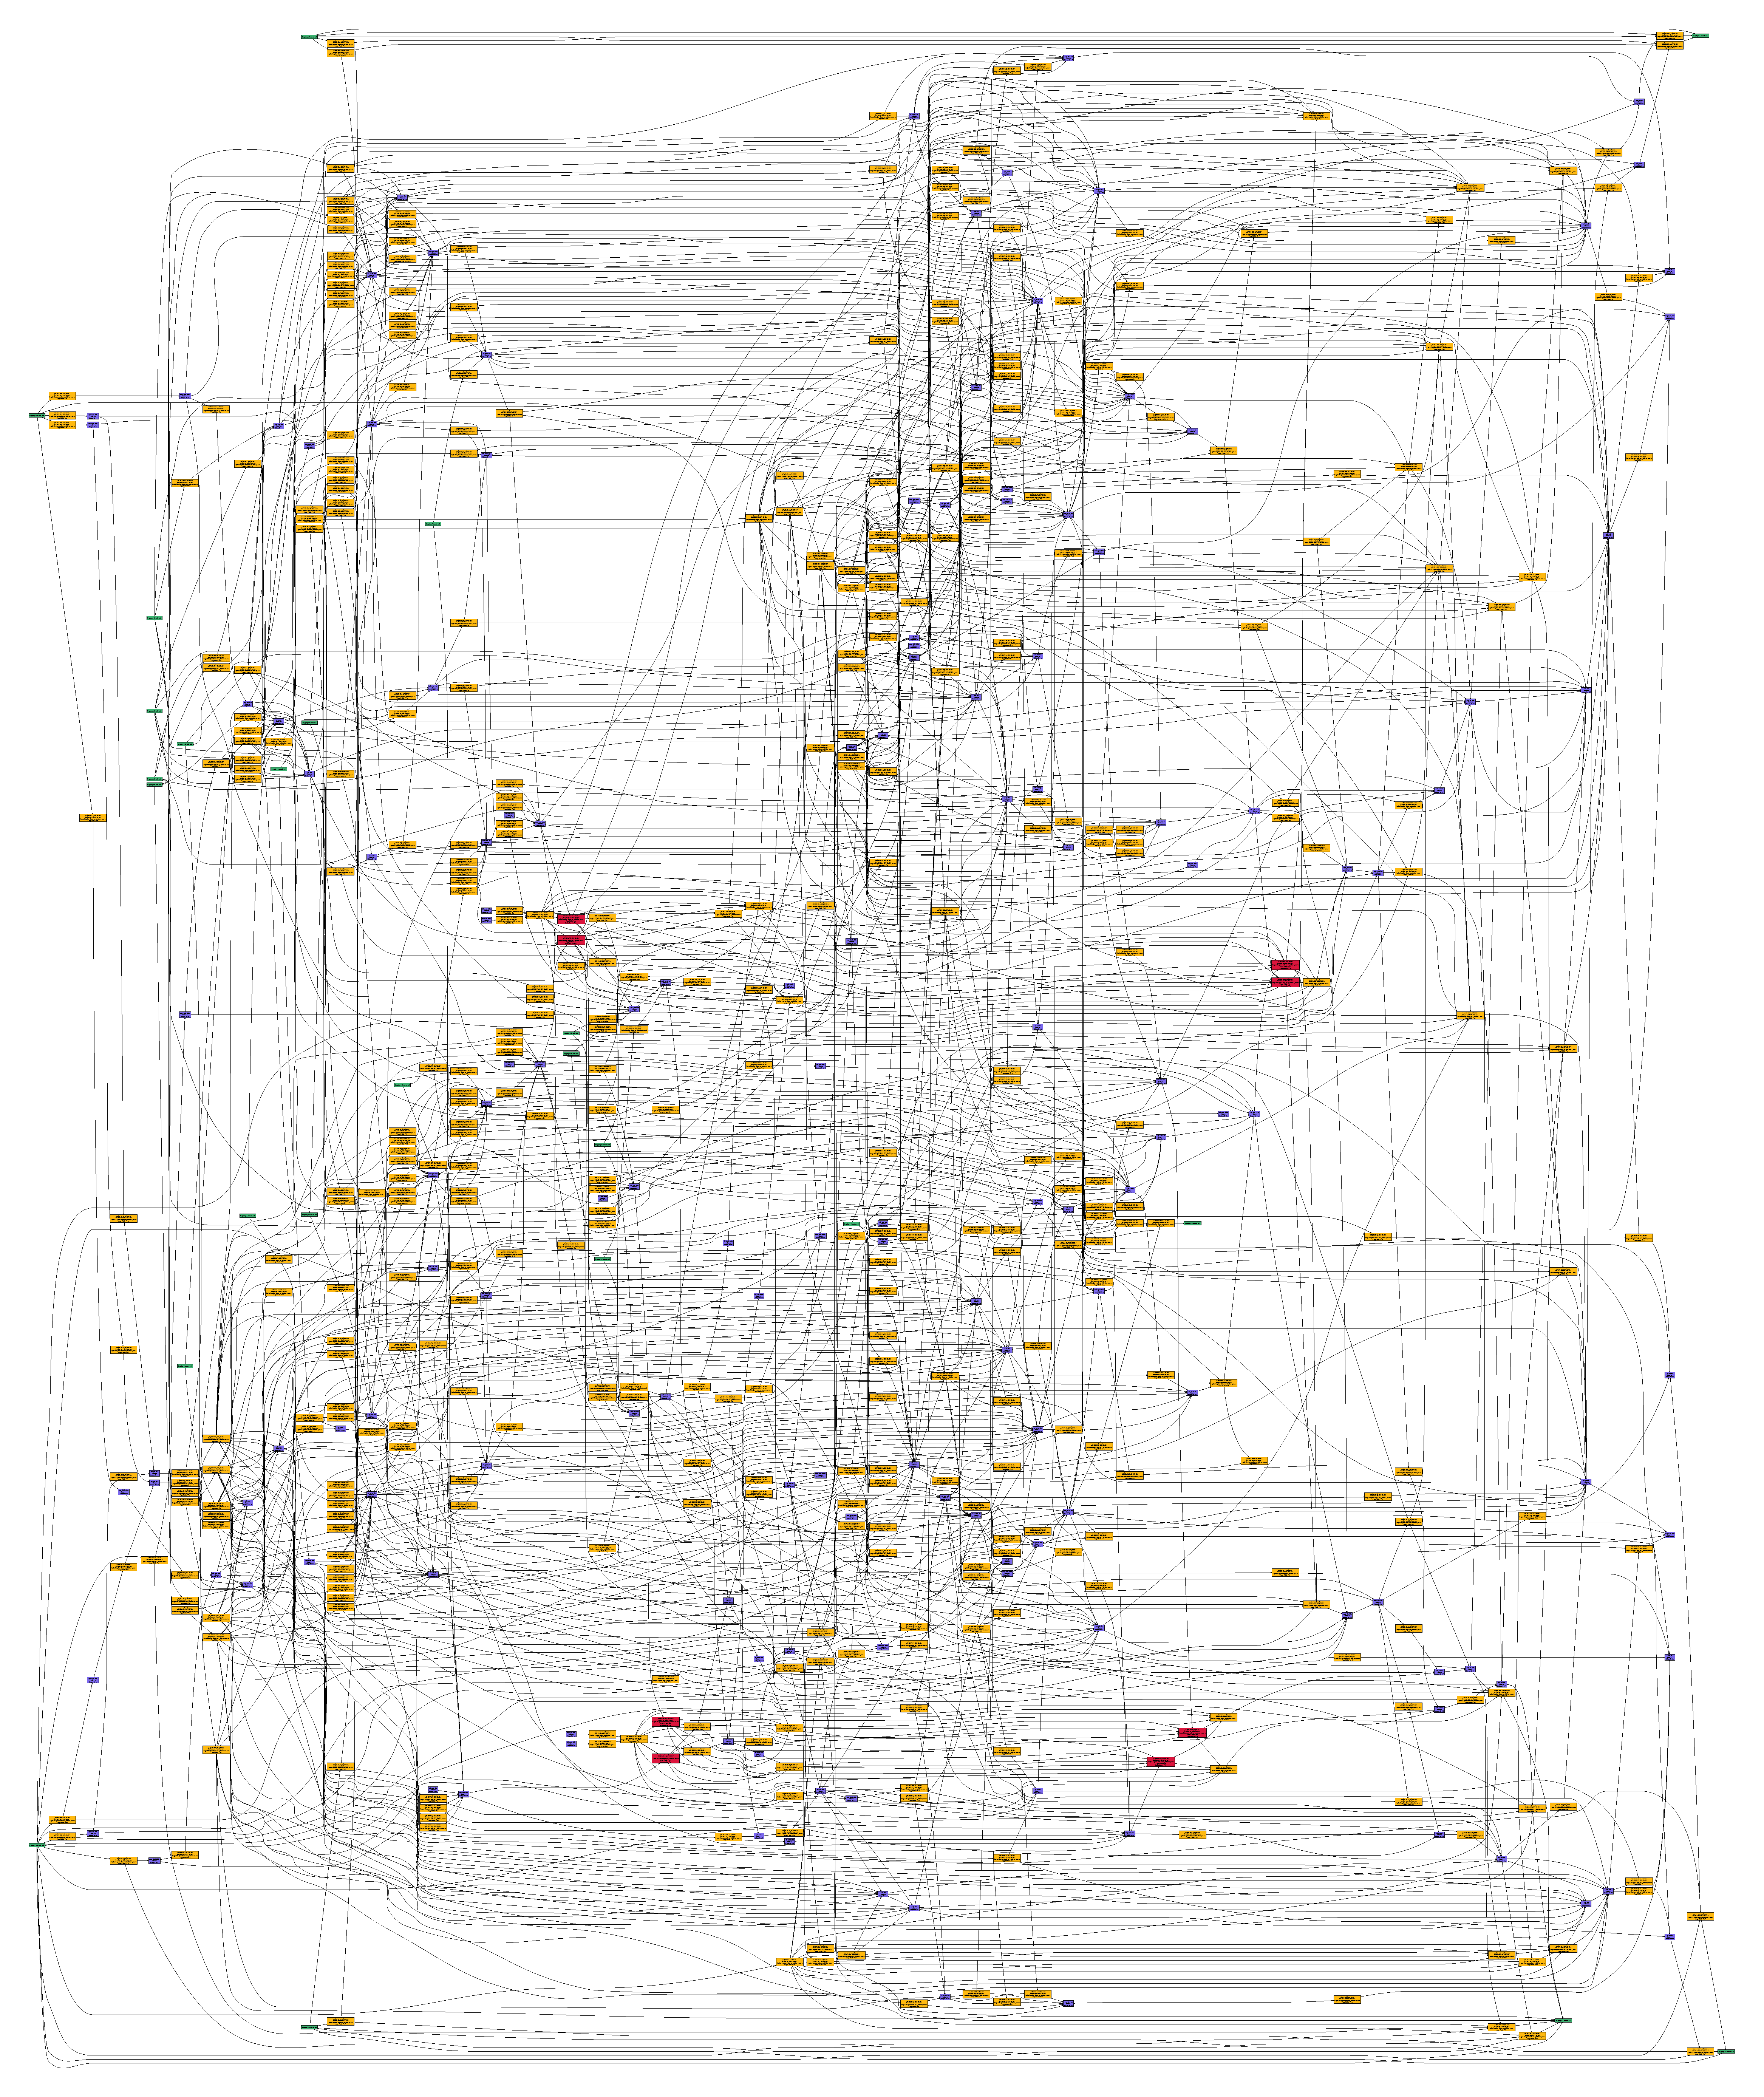
\includegraphics[scale=0.2]{figs/event_graph_example.pdf}
\caption{Example Low-Level Runtime Event Graph from the Pennant Application\label{fig:event_graph_example}}
\end{figure}

Figure~\ref{fig:event_graph_example} shows an example
low-level runtime DAG generated by the high-level runtime 
from a real application. In this image, boxes correspond 
to operations, while edges correspond to event dependences. 
Yellow boxes are copies, red boxes are reductions, 
blue boxes are individual tasks, purple boxes are point 
tasks from an index space task launch, and green boxes 
are inline mappings. This graph shows all of the event
dependences computed by the high-level runtime.
In practice many of these event dependences are pruned
by the high-level runtime through optimizations that
are discussed in Chapter~\ref{chapter:physical}, but
are left in place for the purposes of debugging and
visualization.

While the high-level runtime is responsible for the 
construction of the DAG of operations, the low-level
runtime is responsible for scheduling the operations
onto the target hardware while abiding by the 
constraints specified by event dependences. It is
important to note that many of the DAGs computed
for real applications contain significant amounts of
parallelism.  For example, in 
Figure~\ref{fig:event_graph_example}, the graph is
very tall, indicating that there are many operations
that can be done in parallel as event dependences
primarily point from left to right. By exposing all
of this parallelism in the DAG, the low-level runtime 
can discover significant amounts of work that can
be used to overlap long latency events such as
data movement and synchronization. Most importantly
all of this parallelism is extracted automatically
by the Legion high-level runtime without requiring
any assistance from the programmer. This is only
possible because Legion knows which logical regions
different tasks will be accessing and can therefore safely
infer when tasks and other operations can be 
executed in parallel. In contrast, the burden of 
hiding long latency operations in MPI by overlapping 
computation and communication is placed directly 
on the programmer (see Chapter~\ref{chapter:intro}).

The low-level runtime also serves another
useful purpose in the Legion software stack:
portability.  The low-level runtime interface acts
as an abstraction layer for various hardware interfaces.
The primitives provided by the low-level runtime 
interface are sufficiently simple that they can be
implemented on all current hardware architectures.
Furthermore, their simplicity also suggests that they
should be relatively straightforward to implement on future 
architectures as well.  Consequently, Legion can
easily be ported to both current and future
architectures without needing to re-implement the
entire software stack, but simply by providing
a new low-level runtime implementation that
incorporates new hardware. Since the majority of
Legion code resides in the high-level runtime,
the portability enabled by the low-level runtime
is crucial for making Legion a portable runtime
system.

\subsection{Mapper Interface and Machine Model}
\label{subsec:mapperinst}
The Legion mapping interface is the mechanism by which
Legion applications can directly control how they are 
mapped onto target hardware. As was mentioned in
Section~\ref{subsec:highlevel}, the mapping interface
is actually a reverse interface operated with a 
call-back model.  Whenever mapping decisions need to
be made, the Legion runtime performs a call to
the corresponding mapper object to make the decision.

While mapper functions must always respond to queries, by
associating them with mapper objects, the mapper functions 
are actually methods on mapper objects, permitting mapper
objects to memoize state that can be used for answering
future mapper queries. We discuss details of the various 
mapping queries that can be made and potential 
implementations of them in Chapter~\ref{chapter:mapping}.

In order to aid in making mapping decisions that 
depend on the target architecture, the mapper objects
have direct access to a singleton object called
the {\em machine} object.  The machine object is an
interface for introspecting the underlying hardware
on which the application is executing.  As shown in
Figure~\ref{fig:softwarestack}, the machine object
is provided by the low-level runtime interface directly
to the mapper.  Using the machine object provided by
the low-level runtime, mapper objects can glean 
information about all of the processors and memories
in the system as well as many of their characteristics
such as the latencies and bandwidths for accessing 
or copying data between different memories. Currently,
the machine object is static and does not change
during the duration of an application, but in the
future it may dynamically be modified to reflect the
changing state of hardware (e.g. if a node crashes).
The need to react to such events further underscores
the need for mappers to be dynamic objects capable
of reacting to events at runtime.

\subsection{Runtime and Mapper Instances}
\label{subsec:rtinstances}
Since Legion is designed to operate in a distributed
memory environment, it is useful to understand how 
instances of the Legion runtime and mapper objects 
are deployed throughout the nodes of a machine.  
Figure~\ref{fig:rtinstances} shows where both Legion
runtime instances and mapper instances are instantiated
in a distributed machine with respect to both the
nodes and processors.  An instance of the Legion
high-level runtime is created on every node in the
machine.  This instance of the high-level runtime is
responsible for managing all of the tasks currently
executing on any of the processors on the node. It
is important to note that this approach mandates that
the Legion high-level runtime interface be thread safe 
since tasks running on different processors can invoke 
runtime calls simultaneously.

\begin{figure}[t]
\centering
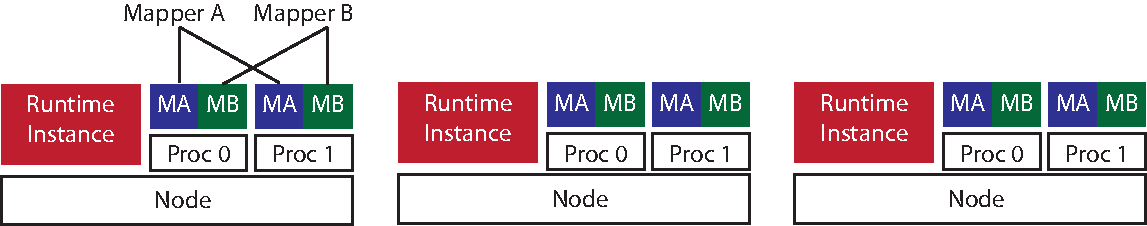
\includegraphics[scale=0.7]{figs/RuntimeInstances}
\caption{Instantiation of Runtime and Mapper Instances\label{fig:rtinstances}}
\end{figure}

In a slightly different manner, mapper objects are
instantiated such that there exists a one-to-one
mapping between mappers and processors on a node. 
Thus, there exists a different mapper object for 
each processor made available by the low-level 
runtime. The reason for this is two-fold.  First, 
by having a unique mapper for each processor, it 
simplifies the process of implementing a Legion 
mapper, as mapper objects can be immediately 
customized for the kind of processor that they 
are managing.  Second, by having separate mappers 
for each processor, we immediately avoid any potential 
sequential bottlenecks because tasks mapping on 
different processors will never conflict with each 
other over a common mapper object. 

\section{Program Execution Framework}
\label{sec:framework}
Having discussed the details of the runtime architecture
we now begin our discussion of the Legion high-level 
runtime and how it executes Legion programs. In 
Chapter~\ref{chapter:model} we described how the
Legion programming model requires all programs to be
described as a tree of tasks that operate on logical
regions. One useful way to conceptualize the execution 
of this tree of tasks is as a hierarchical collection of 
streams of tasks with the execution of each task generating 
a new stream of sub-tasks. To execute each stream of tasks 
we rely on a task pipeline that we introduce in 
Section~\ref{subsec:pipeline}. Section~\ref{subsec:stages}
provides an overview of the different stages in 
the Legion task pipeline. In 
Section~\ref{subsec:hierarchical} we describe
why the hierarchical stream of task abstraction is safe,
allowing streams of tasks with a common parent task
to be considered independently without needing to reason
about interactions with other streams.

\subsection{Out-of-Order Pipeline Analogy}
\label{subsec:pipeline}
The dynamic nature of the Legion runtime requires
efficiency in the analysis of a stream of tasks
because this analysis is overhead that
detracts from the performance of an application.
In order to hide runtime overhead and extract
parallelism from a stream of tasks, Legion 
borrows the idea of an out-of-order
pipeline from hardware architectures and adapts 
it for use within a distributed software environment.
For several decades, hardware designers have relied on 
out-of-order instruction pipelines to both extract 
instruction level parallelism from programs and hide the
overheads associated with dynamic instruction
analysis. Legion applies this abstraction
at the coarser granularity of tasks. The
stream of sub-tasks with region requirements is 
analogous to the stream of instructions with register
names that hardware processors execute.

Our implementation of the Legion runtime exploits this
analogy extensively to both implicitly extract
parallelism from a stream of tasks and to hide the overheads 
associated with dynamic runtime analysis. Many of the
stages of the Legion task execution pipeline described
in Section~\ref{subsec:stages} share obvious analogs
to pipeline stages in traditional out-of-order hardware
processors. The crucial insight that enables this analogy 
is that logical regions provide the necessary information
for describing the data accessed by tasks. As we discuss
in Chapter~\ref{chapter:related}, logical regions 
differentiate the Legion runtime from many of the other
parallel task pipeline systems.

\subsection{Legion Pipeline Stages}
\label{subsec:stages}
Figure~\ref{fig:pipearch} shows the different stages
of the Legion runtime task pipeline\footnote{Some pipeline
stages are interchangeable depending on mapper decisions.
We cover the details of this relationship shortly.}. Each 
task progresses through the stages of the pipeline in order. 
However, the Legion runtime is free to re-order tasks with
respect to each other if tasks are determined to be 
non-interfering. We briefly introduce each of the 
different pipeline stages and where possible describe
analogies to similar stages in hardware out-of-order
processors. The details of many of these stages will
be the subject of later chapters of this thesis.

\begin{figure}[t]
\centering
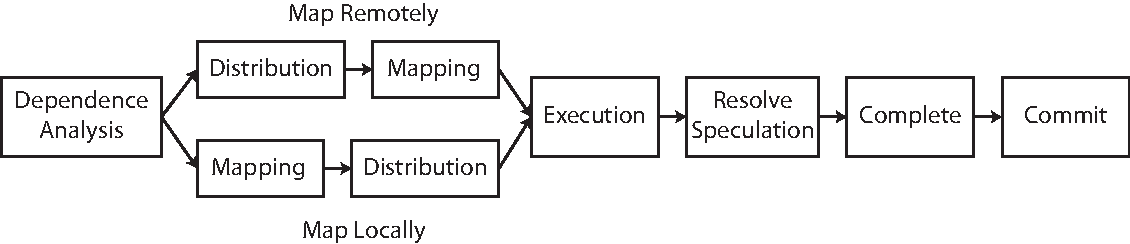
\includegraphics[scale=0.7]{figs/LegionPipeline}
\caption{Legion Runtime Task Pipeline Stages\label{fig:pipearch}}
\end{figure}

The first stage in the Legion task pipeline is dependence
analysis. This stage determines which tasks are safe to
run in parallel and which tasks have dependences based
on logical region usage. Dependence analysis is computed
with respect to the sequential order in which tasks are
issued to the runtime. We refer to this initial order of tasks as 
{\em program order}. Dependences always proceed from tasks coming
earlier in program order to tasks coming later in program
order. The natural partial order on dependences ensures that
deadlock cannot result from the dependence analysis stage.
The dependence analysis stage is similar to the wake-up
select stage of out-of-order processors that decides which
instructions have had all of their dependences satisfied
and are therefore safe to execute. The implementation of
the dependence analysis pipeline stage is covered in 
detail in Chapter~\ref{chapter:logical}.

Once a task has all of its dependences satisfied (because
all of its dependences have mapped), a task progresses
to the mapping phase of the pipeline. The mapping phase
is composed of two tightly coupled stages that are 
interchangeable depending on decisions made by the mapper
for a task. The ordering of the mapping and distribution
stages is determined by whether the mapper wants to map the
task on the node where the task will run, which we call
{\em remote mapping}, or map on the node where the task 
originated, which we call {\em local mapping}. When a task
is remotely mapped, it is first sent to the target node
during the distribution stage along with its meta-data
and then it is mapped during the mapping stage onto
the target processor.  In the case where a task is locally
mapped, it is mapped on the origin node and then sent to
the target node to be executed.  There is an obvious
trade-off to be made by mappers here: mapping remotely
permits more tasks to be mapped in parallel on different 
nodes, but requires movement of meta-data, while locally 
mapping a task does not require meta-data movement, but 
serializes some task mappings. We discuss this trade-off 
in more detail in Chapter~\ref{chapter:mapping}.

While the distribution stage has no obvious analog in
hardware out-of-order processors, the mapping stage
is closely related to the register renaming stage in
hardware processors. In order to permit hardware
processors to extract more instruction level parallelism, 
logical register names are mapped onto a separate set of 
physical registers. Register renaming 
provides an extra level of indirection that allows the 
hardware to remove conflicts such as write-after-read (WAR)
anti-dependences. In Legion, the mapping stage yields
an even more powerful level of indirection. The mapping
stage provides the level of indirection necessary for
decoupling the specification of applications from how
they are mapped onto the target hardware.  During the
mapping stage, mapper objects are queried about how
tasks should be assigned to processors and where physical
instances of logical regions should be placed in the
memory hierarchy. Mapping logical regions onto physical
instances not only allows Legion to remove conflicts
such as WAR anti-dependences on logical regions, but also
allows the mapper to control where instances are placed
in the memory hierarchy for performance. The memory
hierarchy therefore acts as a many-tiered register file
for storing different physical instances of a logical
region. We discuss the implementation of the mapping
stage in Chapter~\ref{chapter:physical} and the 
implementation of the distribution stage in
Chapter~\ref{chapter:distributed}.

The execution stage of the Legion pipeline is nearly
identical to the execution stage for instructions
in hardware processors. In hardware, an instruction
is assigned to an execution unit where it is performed.
In Legion, tasks are assigned to a processor which
then executes the task. The primary difference is
that while instructions in hardware are not capable
of generating new instructions, in Legion, the execution
of a task can generate a new stream of sub-tasks
that then must also be executed by the runtime.
We discuss the implications of the hierarchical
nature of streams of tasks in 
Section~\ref{subsec:hierarchical}.

The fifth stage of the pipeline is used for checking
when speculation has been resolved.  For tasks that 
are not predicated, this stage does not require any
work.  However, for tasks that were predicated and for
which the mapper of the task chose to speculate on
the predicate value (see Section~\ref{subsec:specexec}),
this is the stage where the results of the speculation
are checked.  If a task was correctly speculated, then
this stage performs no work.  However, if the speculation
was incorrect, then work must be performed by the runtime
to either re-execute the task if the speculative value 
of the predicate was incorrectly guessed to be false, 
or the results of the task must be undone if the value 
of the predicate was incorrectly guessed to be true.  
Furthermore, any tasks with dependences upon the 
mis-speculated task must also be rolled back. We 
discuss the details of this process in greater detail 
in Chapter~\ref{chapter:resilience}.

The sixth stage of the pipeline is the completion
stage that determines when a task has finished
executing.  Due to Legion's deferred execution model,
it is possible for a task to finish its execution
stage of the pipeline and continue to progress through
the pipeline while the sub-tasks that it launched
have yet to execute. The completion stage is the
point where a task waits for all of its child tasks
to reach the completion stage. It is important to
note that this definition of completion is inductive: 
in order for a task to complete, all of its descendant 
tasks must already have completed. Once a task is 
complete, it has correctly executed and may propagate 
information such as the result of its future value.  
Tasks that depend on the completion of this task 
are also free to begin executing.  However, for 
resiliency purposes this is not the final stage 
of the pipeline.

The final stage of the pipeline is the commit stage.
The commit stage of the pipeline is used for knowing
when it is safe to reclaim the meta-data associated 
with a task. While a task may have successfully
executed, it is possible that the data generated
by the task is corrupted post execution (e.g. by
a bit-flip in memory). Under these circumstances a task may 
need to be rolled back and re-executed. In order to
perform a roll-back it is necessary to retain the
meta-data (task ID, region requirements, etc.)
for re-executing the task. A task can only be 
committed once we are certain that no roll-back
of the task will ever occur.  We discuss the
conditions for determining when it is safe for a 
task to be committed in Chapter~\ref{chapter:resilience}
and describe how mappers can choose to 
preemptively commit tasks for performance reasons
in Section~\ref{subsec:commit}.

\subsection{Hierarchical Task Execution}
\label{subsec:hierarchical}
As we mentioned in Section~\ref{subsec:stages}, the
Legion pipeline analogy does not directly align with
hardware out-of-order pipelines due to the hierarchical
nature of the Legion programming model.  In a Legion
program the execution of task within the pipeline can
result in an entirely new stream of sub-tasks with
region requirements that need to be executed. The
obvious question then is whether these tasks from 
different streams need to be considered when performing
operations such as dependence analysis and mapping.
Importantly, due to a crucial design decision introduced 
in the Legion programming model, tasks need only consider 
other tasks within the same stream (i.e. originating 
from the same parent task) when progressing through 
the stages of the task pipeline.

Recall from Section~\ref{subsec:subtasks} that a 
task is only permitted to request privileges on 
a subset of the regions and fields for which its
parent task held privileges. This important property
is sufficient to prove a useful theorem: if two tasks
$t_1$ and $t_2$ are non-interfering, then all 
sub-tasks of $t_1$ will be non-interfering with all
sub-tasks of $t_2$.  The proof of this theorem is
based on a formal operational semantics of the Legion
programming model and is beyond the scope of this
thesis.  A full proof of the theorem can be found in
\cite{LegionTypes13}.  

The consequences of this theorem are profoundly
important to the implementation of the Legion runtime.
This theorem permits the Legion runtime to 
implement a hierarchical scheduling algorithm.
Tasks only need to consider other tasks in the
same stream (which all come from the same parent 
task) when traversing the task pipeline. 
Since all tasks in the same stream originate on 
the same node, no communication is 
necessary for performing dependence analysis. 
The hierarchical nature of the Legion task pipeline 
also allows many tasks to be traversing the task 
pipeline in parallel on different nodes. This 
property is essential to enabling Legion to scale 
well on thousands of nodes.

